\documentclass[a2paper, 12pt]{article}
\usepackage[font={huge, bf}]{caption}
\usepackage{fontspec}
\setmainfont{Arial}
\usepackage{subcaption}
\usepackage{graphicx}
\usepackage{tikz}
\usepackage{tikzsymbols}
\usetikzlibrary{calc,patterns,shapes.geometric}
\usepackage{float}
\usepackage{pdflscape}
\usepackage{geometry}
\geometry{landscape, margin=2cm}
\captionsetup[subfigure]{justification=justified,singlelinecheck=false}
\pagestyle{empty}

\def\centerarc[#1](#2)(#3:#4:#5){\draw[#1] ($(#2)+({#5*cos(#3)},{#5*sin(#3)})$) arc (#3:#4:#5);}

\begin{document}
	\vspace*{\fill}
	\begin{figure}[!htbp]
		\centering
		\begin{subfigure}[b]{0.48\textwidth}
			\caption{Figure 1}
			\centering
			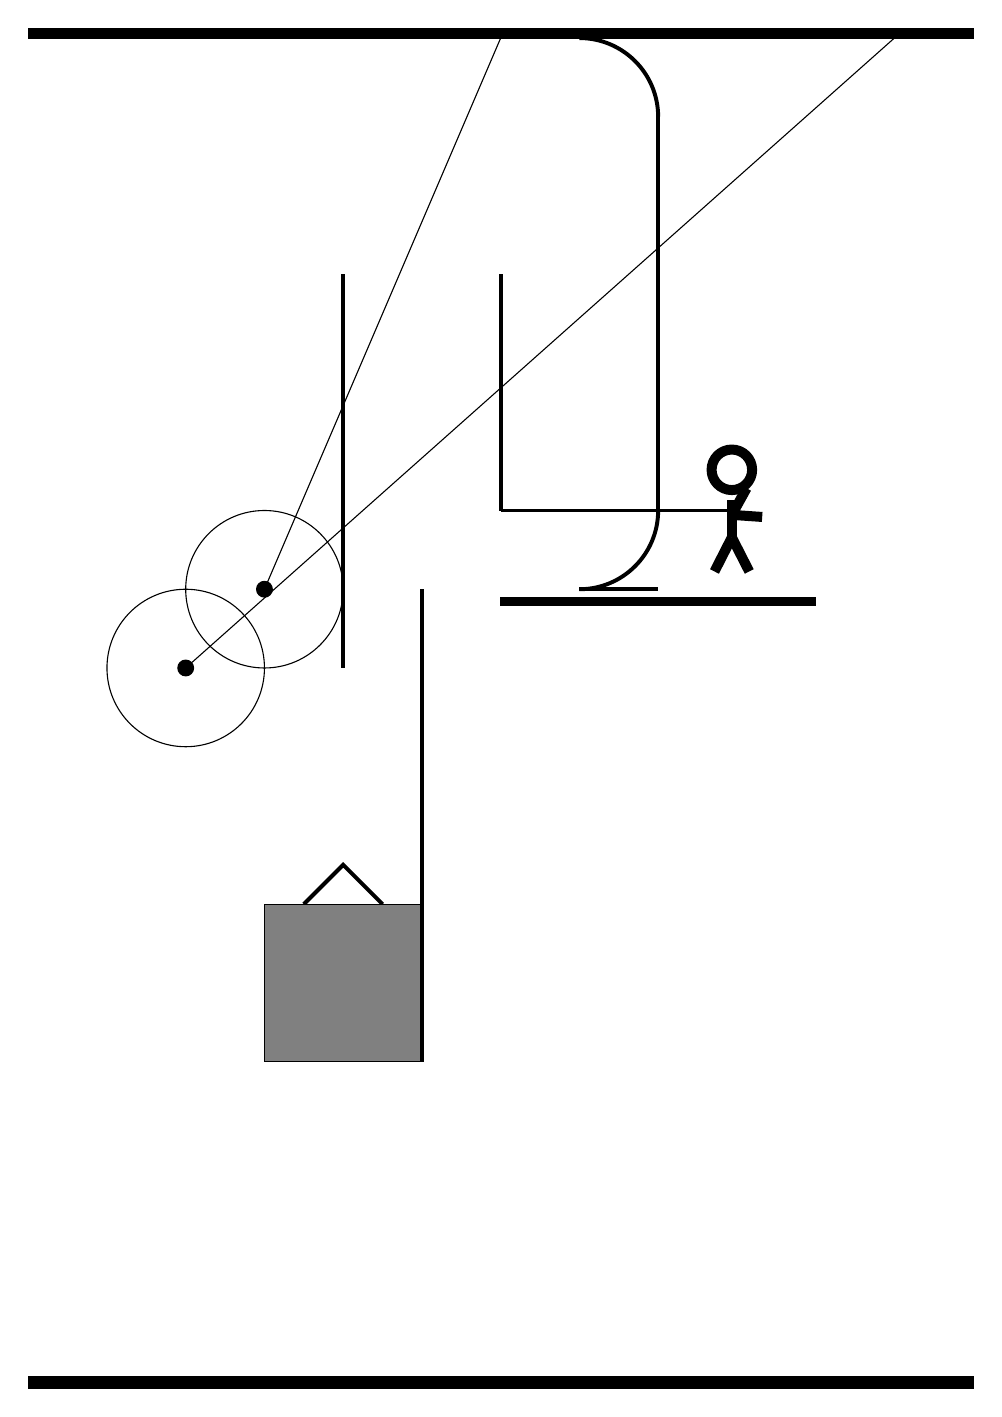
\begin{tikzpicture}
				\draw[fill=black] (-4, 14) rectangle (8, 14.125);
				
				\draw (-1,7) circle (1);
				\draw[fill=black] (-1,7) circle (0.1);
				\draw (2,14.0) -- (-1,7);
				
				\draw (-2,6) circle (1);
				\draw[fill=black] (-2,6) circle (0.1);
				\draw (7,14.0) -- (-2,6);
				
				\draw[line width=0.5mm](-0.5,3) --  (0,3.5) -- (0.5,3);
				\draw[fill=black!50] (-1, 3) rectangle (1, 1);
				
				\draw[line width = 0.5mm] (3,7) arc (270:360:1);
				\draw[line width = 0.5mm] (4,8) -- (4,13);
				\draw[line width = 0.5mm] (4,13) arc (0:90:1);
				\draw[line width = 0.5mm] (0,6) -- (0,11);
				\centerarc[line width = 0.5mm](1,11)(0:180:1);
				\draw[line width = 0.5mm] (2,11) -- (2,8);
				\centerarc[line width = 0.5mm](3,8)(270:180:1);
				\draw[line width = 0.5mm] (3,7) -- (4,7);
				\draw[line width = 0.5mm] (2,8) -- (5,8);
				\centerarc[line width = 0.5mm](2,7)(90:180:1);
				\draw[line width = 0.5mm] (1,7) -- (1,1);
				
				\node at (5, 8) {\scriptsize \Strichmaxerl[10][-119][-4]};
				\draw[fill=black] (2, 6.9) rectangle (6, 6.8);
				
				\draw[fill=black] (-4, -3) rectangle (8, -3.15);
			\end{tikzpicture}
		\end{subfigure}
		\hfill
		\begin{subfigure}[b]{0.48\textwidth}
			\caption{Figure 2}
			\centering
			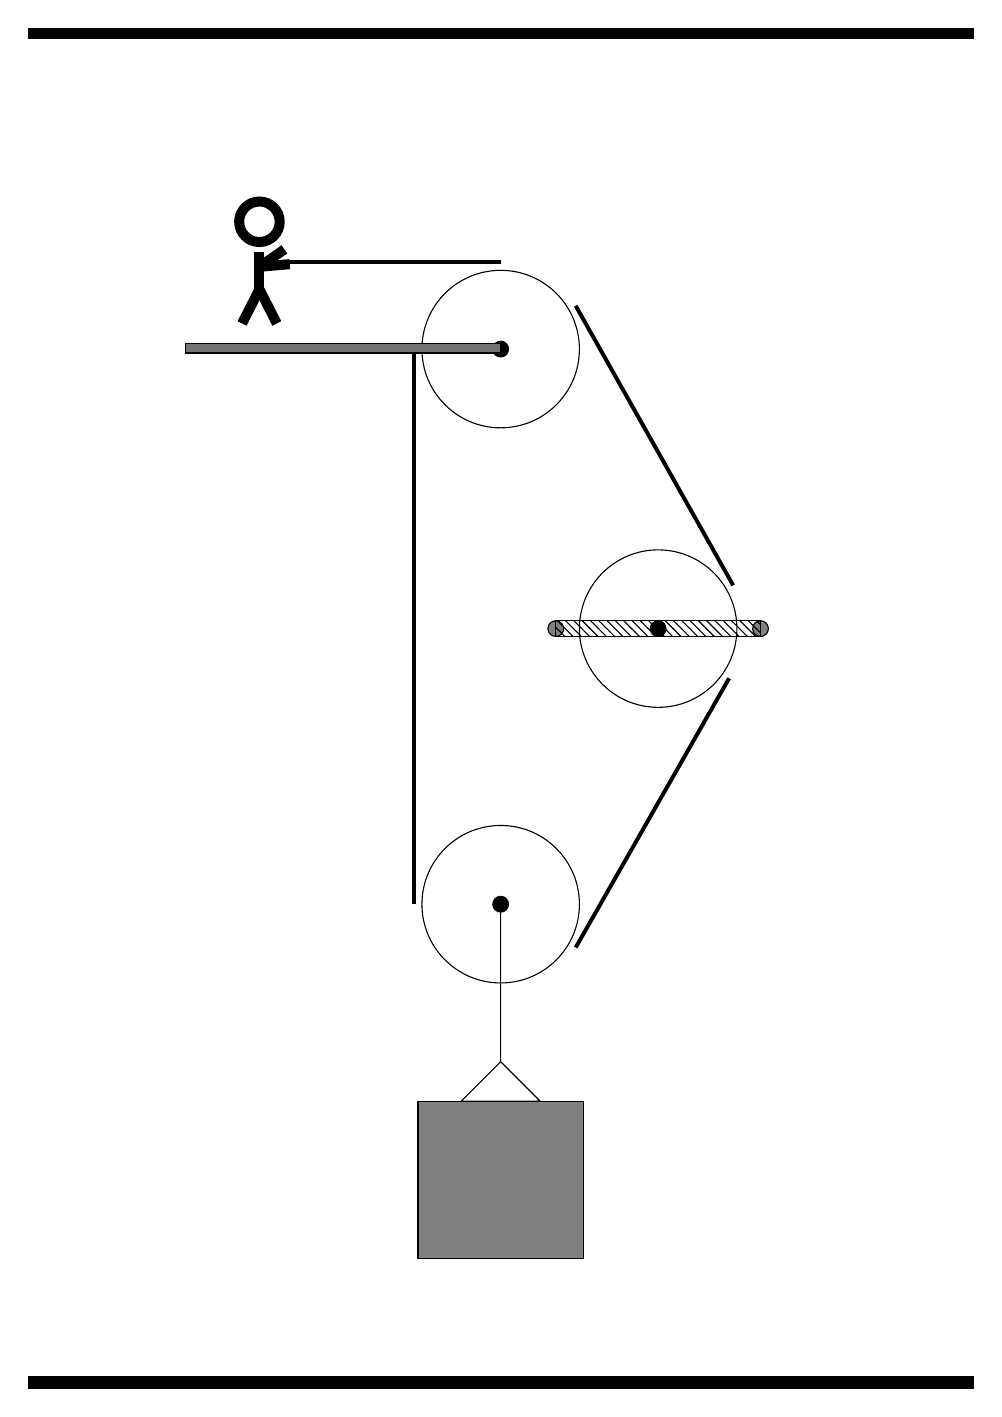
\begin{tikzpicture}
				\draw[fill=black] (-4, 14) rectangle (8, 14.125);
				
				\draw (2, 3.0) circle (1);
				\draw[fill=black] (2, 3.0) circle (0.1);
				
				\draw (2, 10.05) circle (1);
				\draw[fill=black] (2, 10.05) circle (0.1);
				
				\draw[fill=white](4, 6.5) circle (1);
				\draw[fill=black] (4, 6.5) circle (0.1);
				\draw[fill=black!50] (2.7, 6.5) circle (0.1);
				\draw[fill=black!50] (5.3, 6.5) circle (0.1);
				\draw[pattern=north west lines, pattern color=black] (2.7, 6.6) rectangle (5.3, 6.4);
				
				\draw (2, 3.0) -- (2, 1.0) -- (1.5, 0.5) -- (2.5, 0.5) -- (2, 1.0);
				\draw[fill=black!50] (0.95, 0.5) rectangle (3.05, -1.5);
				
				\draw[line width=0.5mm] (0.9, 10) -- (0.9, 3.0);
				\centerarc[line width=0.5mm](2, 3.0)(180:330:1.1);
				\draw[line width=0.5mm](2.9526, 2.45) -- (4.9011, 5.869);
				\centerarc[line width=0.5mm](4, 6.5)(390:325:1.1);
				\draw[line width=0.5mm](4.9526, 7.05) -- (2.9526, 10.6);
				\centerarc[line width=0.5mm](2, 10.05)(30:90:1.1);
				\draw[line width=0.5mm](2, 11.15) -- (-1, 11.15);
				
				\node at (-1, 11.15) {\scriptsize \Strichmaxerl[10][-175][35]};
				\draw[fill=black!55] (-2, 10) rectangle (2, 10.125);
				
				\draw[fill=black] (-4, -3) rectangle (8, -3.15);
			\end{tikzpicture}
		\end{subfigure}
	\end{figure}
		\vspace*{\fill}
\end{document}